\documentclass[tikz,convert={outfile=\jobname.svg}]{standalone}
\usetikzlibrary{arrows.meta}
\begin{document}
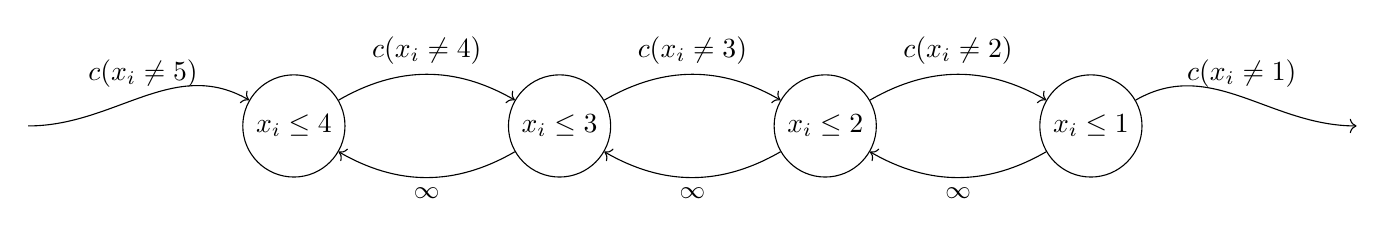
\begin{tikzpicture}[x=80pt, y=80pt]
    \node[draw=black, fill=white, circle, minimum size=30pt] at (-1.8,0) (x_4) {$x_i \le 4$};
    \node[draw=black, fill=white, circle, minimum size=30pt] at (-0.6,0) (x_3) {$x_i \le 3$};
    \node[draw=black, fill=white, circle, minimum size=30pt] at (0.6,0) (x_2) {$x_i \le 2$};
    \node[draw=black, fill=white, circle, minimum size=30pt] at (1.8,0) (x_1) {$x_i \le 1$};

    \draw[->] (x_3) to[out=-150, in=-30] node[below] {\small $\infty$} (x_4);
    \draw[->] (x_2) to[out=-150, in=-30] node[below] {\small $\infty$} (x_3);
    \draw[->] (x_1) to[out=-150, in=-30] node[below] {\small $\infty$} (x_2);
    \draw[->] (-3,0) to[out=0, in=150] node[above] {$c(x_i \ne 5)$} (x_4);
    \draw[->] (x_4) to[out=30, in=150] node[above] {$c(x_i \ne 4)$} (x_3);
    \draw[->] (x_3) to[out=30, in=150] node[above] {$c(x_i \ne 3)$} (x_2);
    \draw[->] (x_2) to[out=30, in=150] node[above] {$c(x_i \ne 2)$} (x_1);
    \draw[->] (x_1) to[out=30, in=180] node[above] {$c(x_i \ne 1)$} (3,0);
\end{tikzpicture}
\end{document}
